\section{Parallelism \weekDoran{4}}
	\subsection{Coprocessors \weekPageDoran{4}{6-7}}
	
		Classical coprocessors have their own instruction set. The use of the device is triggered by co-processor instructions in the programme code. The co-processor generally has some form of exception registration.
		
		\vspace{0.5cm}
		
		\textbf{Example mechanism:}
		
		\begin{enumerate}
		  \item Processor receives unidentified instruction.
		  \item Processor asks its co-processors whether this instruction applies to them.
		  \begin{enumerate}
			  \item If it doesn't, the processor raises an unidentified op-code exception and let normal processing take over.
			  \item If it does, the instruction is passed to the co-processor which then executes it.
			  \item If the co-processor is busy while the processor has a co-processor instruction lined up, the processor will stall.
		  \end{enumerate}	  
		  \item The processor will continue to execute instructions while the co-processor does the same with the passed instruction.
		\end{enumerate}


		\begin{table}[H]
			\centering
			\begin{tabular}{|p{0.425\textwidth}|p{0.425\textwidth}|}
				\hline
				\textbf{Loosely Coupled Co-Processors}
					& \textbf{Loosely Coupled Co-Processors}\\
				\hline
				Access to memory and external resources via system bus.
					& Access to memory and external resources via specialised interface.\\
				\hline
			\end{tabular}
		\end{table}
		
	\subsection{Pipelines \weekPageDoran{4}{8-29}}
	
		\begin{tabular}{cc}
			\begin{minipage}{0.475\textwidth}
				\begin{figure}[H]\centering
					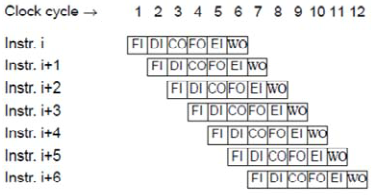
\includegraphics[width=\textwidth]{./pictures/pipelining.png}
				\end{figure}
			\end{minipage}
			&	
				\begin{minipage}{0.475\textwidth}
					\begin{table}[H]
						\centering
						\begin{tabular}{|>{\bfseries}l|l|}
							\hline
							\multicolumn{2}{|c|}{\textbf{Pipeline Legend}}\\
							\hline
							FI
								& Fetch instruction\\
							\hline
							DI
								& Decode instruction\\
							\hline
							CO
								& Calculate operand address\\
							\hline
							FO
								& Fetch operand\\
							\hline
							EI
								& Execute instruction\\
							\hline
							WO
								& Write operand\\
							\hline
						\end{tabular}
					\end{table}		
				\end{minipage}\\
		\end{tabular}
		
		\subsubsection{CISC vs. RISC Architecture}
		\begin{table}[H]
			\centering
			\begin{tabular}{|p{0.425\textwidth}|p{0.425\textwidth}|}
				\hline
				\textbf{RISC}
					& \textbf{CISC}\\
				\hline
				Reduced Instruction Set Computing
					& Complex Instruction Set Computing\\
				\hline
				Each instruction is divided in different sub-instructions. These sub-instructions are kept separately, therefore the circuitry is much simpler.
					& Each instruction is actually a series of operations. E.g. loading input, performing the operation and storing the result.\\
				\hline
				Each instruction can be completed in one clock cycle.
					& Execution time of an instruction depends largely on where data is stored and many other factors.\\
				\hline
			\end{tabular}
		\end{table}		
		
		For CISC-processors, separate hardware blocks are used for each instruction. Therefore it is possible to assign a hardware block for each sub-instruction which does its job and is then idle until the same sub-instruction of the next instruction comes along. Thus, this architecture allows for pipelining.
		
		\subsubsection{Hazards}
			\begin{longtable}{|>{\bfseries}p{0.09\textwidth}|p{0.4\textwidth}|p{0.46\textwidth}|}
				\hline
				Structural Hazards
					& \textbf{Occurs because} resource is requested by more than one instruction at the same time.\newline
						\textbf{E.g.:} Memory cannot accept another transfer within a clock cycle.\newline
						\textbf{Possible resolutions:} Duplicate resources, pipeline functional units too (e.g. ALU, Floating point unit..)
						
					& \vspace{0pt}
					
						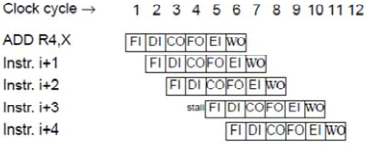
\includegraphics[width=0.45\textwidth]{./pictures/structuralHazard.png}\\
				\hline
				Data\newline Hazards
					& \textbf{Occurs because} if next instruction depends on result of previous instruction.\newline 
						\textbf{Possible resolutions:} Using a technique called forwarding/bypassing: Result of previous instruction will be forwarded directly to where the next instruction needs it, instead of stalling until the previous instruction writes back the result.
					& \vspace{0pt}
					
						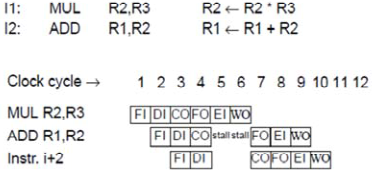
\includegraphics[width=0.45\textwidth]{./pictures/dataHazard.png}\\
				\hline
				Control Hazards
					& \textbf{Occurs because} of branch instructions .\newline
						\textbf{E.g.:} It is unknown that a branch instruction was fetched before it is decoded. At this point the instructions that followed the branch instruction in memory were already fetched and decoded, but these instructions are not executed.\newline
						\textbf{Possible resolutions:} Several approaches, e.g. branch prediction(use statistics to predict branch outcome)
					& \vspace{0pt}
					
						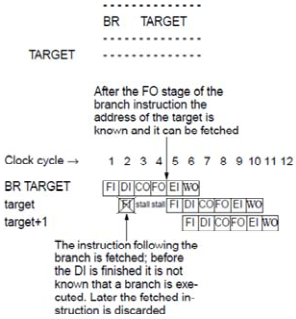
\includegraphics[width=0.45\textwidth]{./pictures/controlHazard.png}\\
				\hline
			\end{longtable}
		